\documentclass{article}
\usepackage[a4paper, total={6in, 8in}]{geometry}
\usepackage{graphicx}
\usepackage{url}
\usepackage{natbib}
\usepackage{todonotes}
\usepackage{booktabs}
\usepackage{lineno}
\usepackage{color}
%\usepackage{auto-pst-pdf}
\usepackage[colaction]{multicol}
\usepackage{caption}
\usepackage{svg}
\usepackage{authblk}
\usepackage{standalone}
\usepackage[section]{placeins}

\usepackage{xr}
\externaldocument{main}

\makeatletter
\renewcommand{\maketitle}{\bgroup\setlength{\parindent}{0pt}
	\begin{flushleft}
		
		{\huge\textbf{\@title}}
		
		\bigskip
		
		{\large\textbf{\@author}}
		
		\bigskip
		
		{\large{ \@date}}
		
	\end{flushleft}\egroup
}
\makeatother


\begin{document}
	% Title
	\title{A Topic Model of Climate Change Literature}
	\title{Words, words, words: Mapping the Matter of Climate Change Literature}
	\title{A Topography of Climate Change Research}
	
\author[1,2]{Max Callaghan*}
\author[1,2]{Jan Minx}
\author[2]{Piers M. Forster}

\affil[1]{Mercator Research Institute on Global Commons and Climate Change, Torgauer Straße, 10829 Berlin, Germany}
\affil[2]{Priestley International Centre for Climate, University of Leeds, Leeds LS2 9JT, United Kingdom}
	\maketitle
	\section*{Extended Figures}
			\setcounter{figure}{0}


\begin{figure}
	\begin{center}
		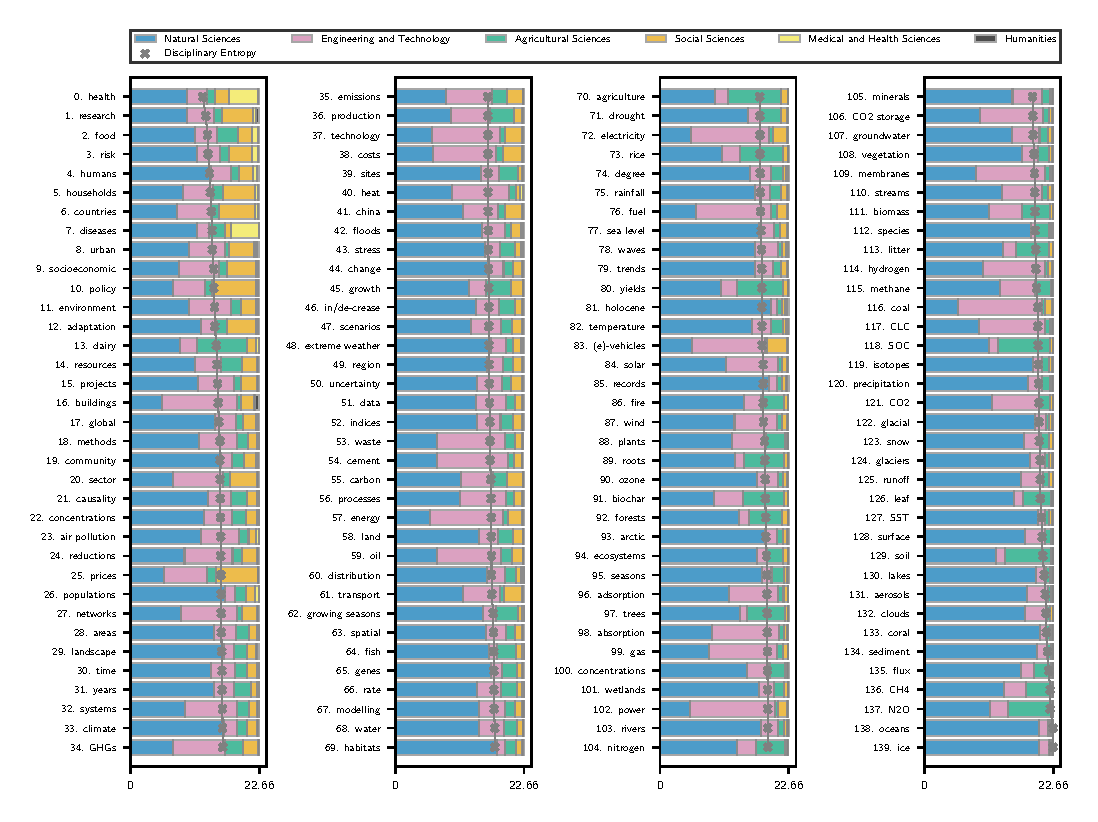
\includegraphics[width=1\linewidth]{../plots_pub/topic_oecd_entropy.pdf}
		\caption{Disciplinary Entropy of Topics. Coloured bars show the proportion of each topic made up of papers from each disciplinary category. Crosses show the Disciplinary Entropy of each topic (see methods for details).}
		\label{dis-entropy}
	\end{center}
\end{figure}	



\begin{figure}
	\begin{center}
		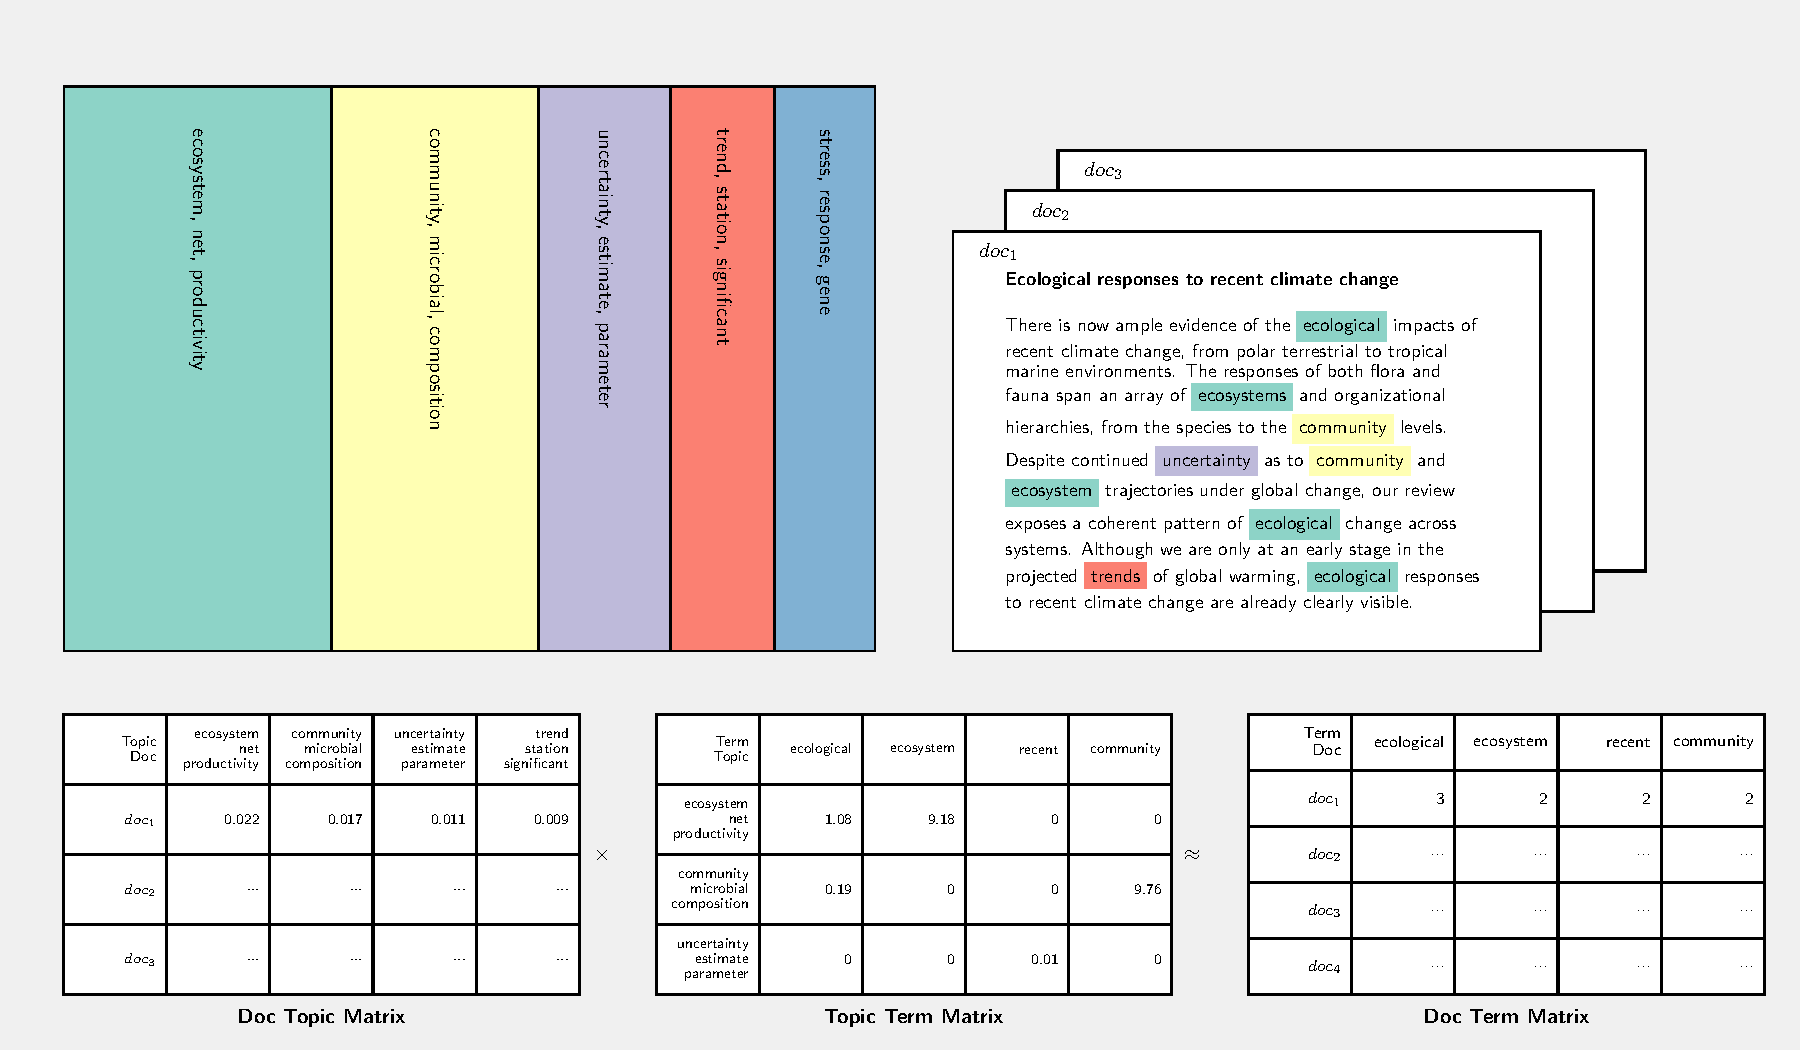
\includegraphics[width=1\linewidth]{../plots_pub/single_doc_3_536594_1861.pdf}
		\caption{Topic make up of a single document. The Doc Term Matrix shows the number of occurrences of each term in the document. The Topic Term Matrix shows the topic score of each term-topic combination. The Doc Topic Matrix shows the document-topic score for each topic. This topic makeup of the document shown is illustrated by the bars in the top left. Words highly associated with each topic that occur in the document are highlighted. All values are real, although the doc-term matrix is scaled by the inverse-document frequency before being used in the model.}
		\label{doc-topic}
	\end{center}
\end{figure}

\begin{figure}
	\begin{center}
		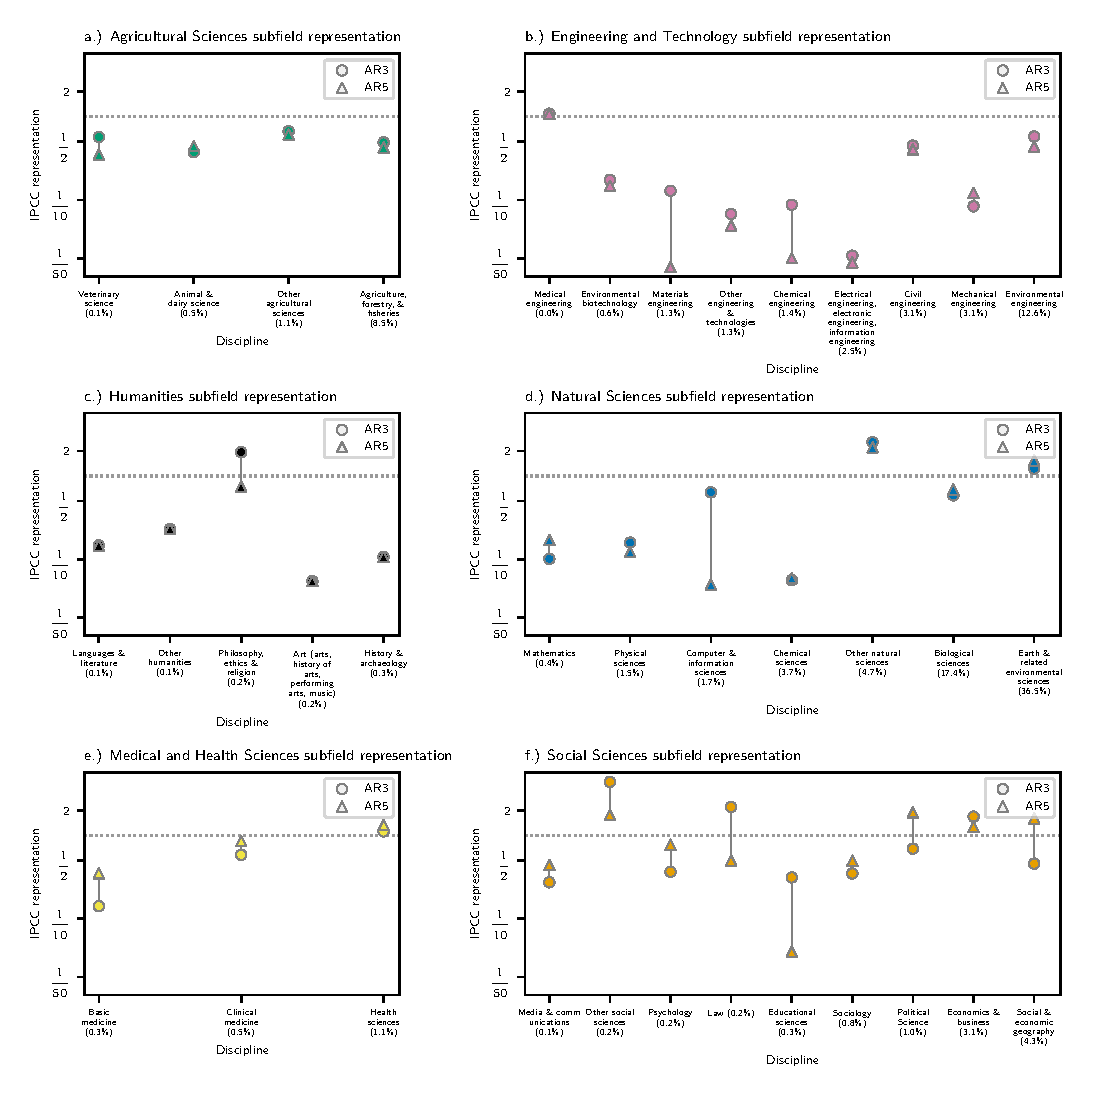
\includegraphics[width=1\linewidth]{../plots_pub/ipcc_rep_wcs_simplified.pdf}
		\caption{IPCC Representation by subfield. Representation is the share of the subset of documents being cited by the IPCC divided by the share of the subset in the whole literature. We plot on a log scale so that 0.5 is equally distant to 1 as 2; plot labels show real values.}
		\label{subfield}
	\end{center}
\end{figure}

\begin{figure}
	\begin{center}
		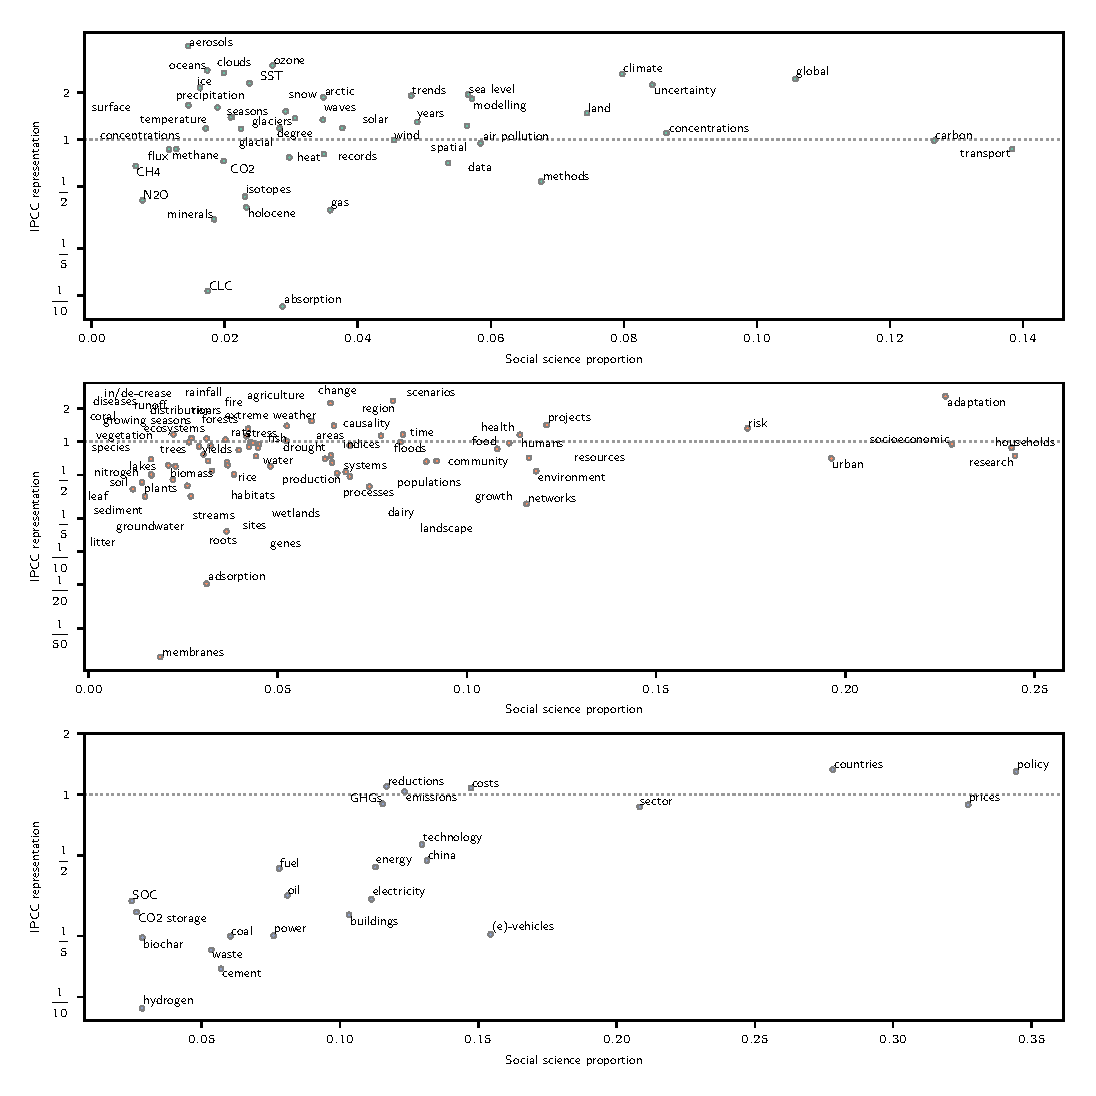
\includegraphics[width=1\linewidth]{../plots_pub/wgs_socsci.pdf}
		\caption{SI Social science \& representation in topics across working groups. Representation is the share of the subset of documents being cited by the IPCC divided by the share of the subset in the whole literature. Social science proportion shows the proportion of the total document-topic score coming from documents in the social sciences.}
		\label{socsci-wgs}
	\end{center}
\end{figure}

\begin{figure}
	\begin{center}
		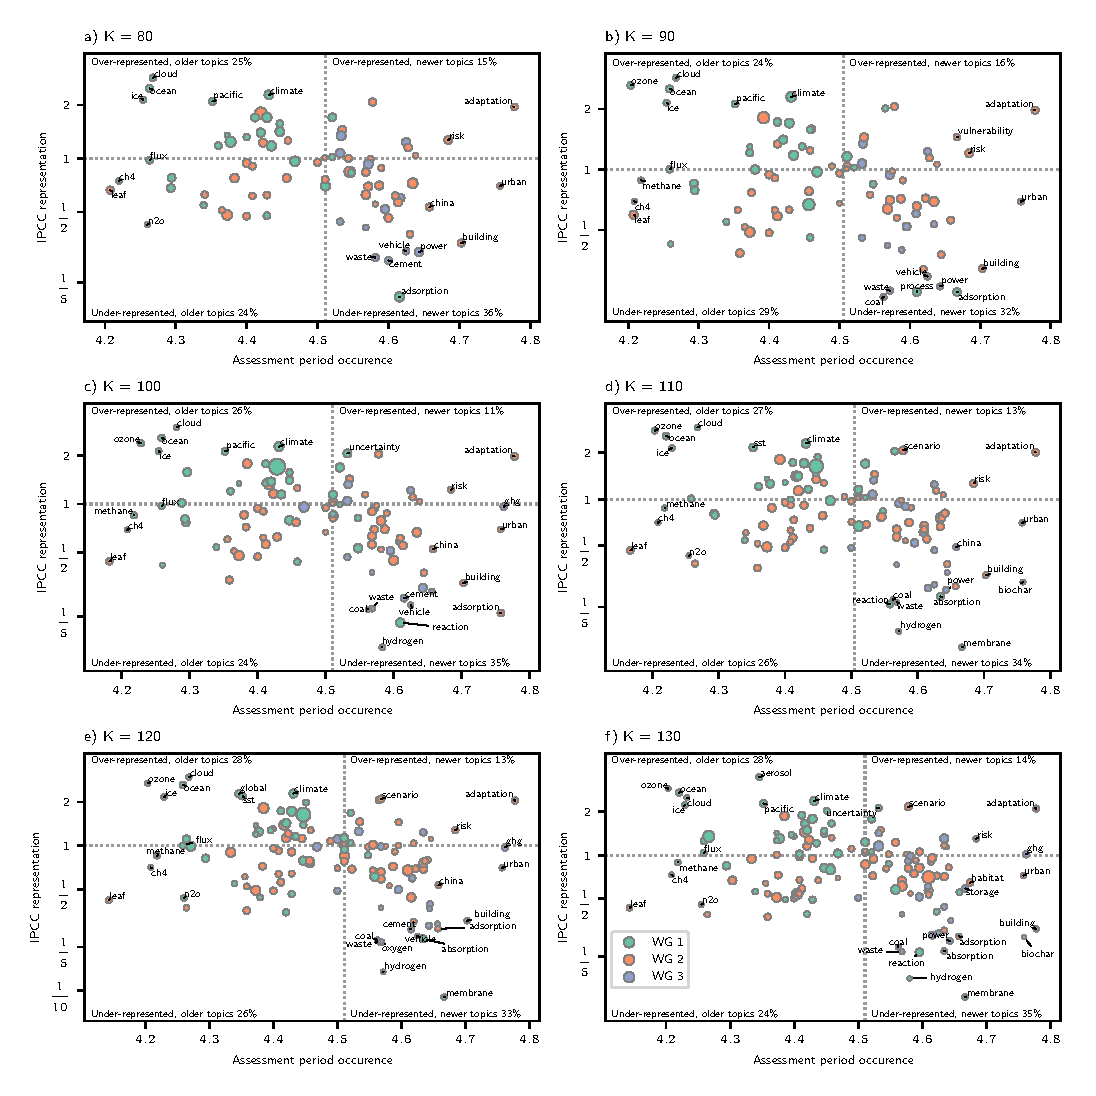
\includegraphics[width=1\linewidth]{../plots_pub/topic_rep_ks.pdf}
		\caption{Topic representation over different values of K (number of topics). Topics in the upper or lower 6.66th percentile of either dimension are labelled. Representation is the share of the subset of documents being cited by the IPCC divided by the share of the subset in the whole literature. Assessment period occurrence refers to the center of a topic's distribution across assessment periods (see methods for further details).}
		\label{top-rep-ks}
	\end{center}
\end{figure}

\end{document}